\section{Sorting}
\label{sec:sorting}

One of the most fundamental operations in computer science is sorting a sequence of elements. And as old as the problem is as numerous are the algorithms to solve it. These sorting algorithms differ in various aspects such as best, average and worst runtime or memory complexity, stability, the number of comparisons and swaps and whether the algorithm is a comparison sort or not.

The sort implementations provided by todays standard libraries are highly tuned achieving an optimal asymptotic runtime complexity which is $\mathcal{O}(n log n)$ for comparison based sorts. Examples would be variations of quick sort (C), merge sort (C++), intro sort (C++, .NET) or Timsort (Java, Python). All these algorithms are comparison sorts, thus requiring a method of comparing two elements of the input sequence. This comparison is often provided either by the language or standard library (e.g. $<$ operator) or by the programmer via a custom comparison function giving the flexibility to compare and sort any kind of elements.

Another class of sorting methods are integer sorting algorithms. These algorithms do not use comparisons to determine the order of elements but rely on more flexible integer arithmetic applied to the keys which should be sorted. Therefore, they can achieve a better asymptotic runtime complexity than comparison based ones. Popular algorithms of this kind are radix sort, counting sort and bucket sort. All of them running with $\mathcal{O}(n + k)$ or $\mathcal{O}(n * k)$ (where k is a constant) in linear time.
However, despite their key limitation, integer sorting algorithms also work on other kind of types as long as they can be represented as integers in binary (e.g. strings can be seen as byte array forming a (larger) integer).

Considering parallelizability and an eventual GPU implementation, sorting lies between matrix multiplication and prefix sum offering some degree of parallelism depending on the chosen algorithm. The following chapter will focus on the implementation of two widely chosen algorithms for GPU sorting. These are the comparison based bitonic sorting network and the integer sorting algorithm radix sort. To reduce code complexity (especially of the latter), the input array consists of unsigned 32 bit integers.


\subsection{CPU Implementations}

\subsubsection{C/C++ standard library routines}

As the later GPU implementations should be compared with well implemented and wide-spread CPU ones, the first step is to measure the performance of the standard library's routines.
Listing \ref{lst:sort_cpu_qsort} shows a typical usage of the \lstinline|qsort()| function provided by the stdlib header from C.

\lstset{basicstyle=\ttfamily{}\scriptsize{}}
\lstinputlisting[language=C++, caption=Sorting an array of unsigned integers using \lstinline!qsort()! from the C stdlib header., label=lst:sort_cpu_qsort, firstline=36, lastline=46]{code/sort/main.cpp}
\lstset{basicstyle=\ttfamily{}}

As qsort() is usually precompiled and part of the runtime library, a compare function has to be provided which is called for every comparison. This will probably slow down the run time when compared with the C++ \lstinline!std::sort()! which can use an existing overload of the $<$ operator or inline a provided compare function thanks to templates.
Listing \ref{lst:sort_cpu_sort} shows a typical call to the \lstinline!std::sort()! function template from the C++ algorithm header.

\lstset{basicstyle=\ttfamily{}\scriptsize{}}
\lstinputlisting[language=C++, caption=Sorting an array of unsigned integers using \lstinline!std::sort()! from the C++ algorithm header., label=lst:sort_cpu_sort, firstline=48, lastline=51]{code/sort/main.cpp}
\lstset{basicstyle=\ttfamily{}}

As the $<$ operator is defined for unsigned integer types no custom compare function has to be provided and no additional overhead is created for comparing elements.
The difference can be clearly seen in the benchmark chart in figure \ref{fig:sort_chart}. It takes \lstinline!qsort()! 14.746 seconds to sort a sequence of $2^{26}$ elements while \lstinline!std::sort()! only requires 9.039 seconds.

\subsubsection{Radix sort}
\label{sec:sorting_radix_cpu}

In contrast to the comparison based \lstinline!qsort()! and \lstinline!std::sort()! radix sort operates on the binary representation of the input elements in several passes. Originally, in each pass a bit of each input element is selected (starting with the least significant bit). The input elements are then split into two sequences (called buckets) according to the selected bit. This is done by creating a histogram holding the number of elements having the same bit value for each bit combination (0 or 1). After the histogram has been created it is exclusively scanned. The scanned histogram now holds the start index for each bucket. The input elements are permuted and moved into their corresponding buckets according to the selected bit. Elements with an equal bit are written into the same bucket in the same order as they appeared in the pass' input (each pass is stable). An auxiliary array is usually needed for this permute step. This procedure is repeated for every bit of the input elements. 

By only selecting one bit in each pass 32 passes are required to sort the input sequence (elements are 32 bit unsigned integers). In each pass the input array is iterated over two times and the histogram has to be scanned once. This accumulates to 64 iterations over the input sequence and 32 scans of a two element histogram making radix sort a linear algorithm but with a quite significant constant factor. This factor can be reduced by selecting several bits of each input element at once in each pass. As a result the number of passes decrease linearly with the number of selected bits (which is called radix and gives the algorithm its name). As a trade-off the size of the histogram increases by a power of two.

The CPU radix sort implementation used in the benchmarks is provided in listing \ref{lst:sort_cpu_radix}.

\lstset{basicstyle=\ttfamily{}\scriptsize{}}
\lstinputlisting[language=C++, caption=Sorting an array of unsigned integers using radix sort. The algorithm uses eight passes analyzing four bits each. The implementation is based on the radix sort sample shipped with AMD APP SDK \cite{amd_app_sdk}., label=lst:sort_cpu_radix, firstline=53, lastline=105]{code/sort/main.cpp}
\lstset{basicstyle=\ttfamily{}}

The implementation uses a relatively high radix of 16 (\lstinline!RADIX!) which allows radix sort to finish in two passes. As a consequence, the histogram consists of $2^{16}$ elements (\lstinline!BUCKETS!) occupying 256 KiB of memory but has to be scanned only two times.

The performance difference of radix sort to the previously presented comparison based algorithm is significant as seen in figure \ref{fig:sort_chart}. Although the high radix of 16 causes a large overhead on small input sizes (as the full $2^{16}$ element histogram has to be scanned independently of the input size), radix sort shows its strength on larger inputs. It catches up to \lstinline!std::sort()! at approximately 10,000 elements and then outdistances the library routine largely sorting $2^{26}$ elements in 0.884 seconds (compared to 9.039 seconds of \lstinline!std::sort()!).

\begin{figure}
\centering
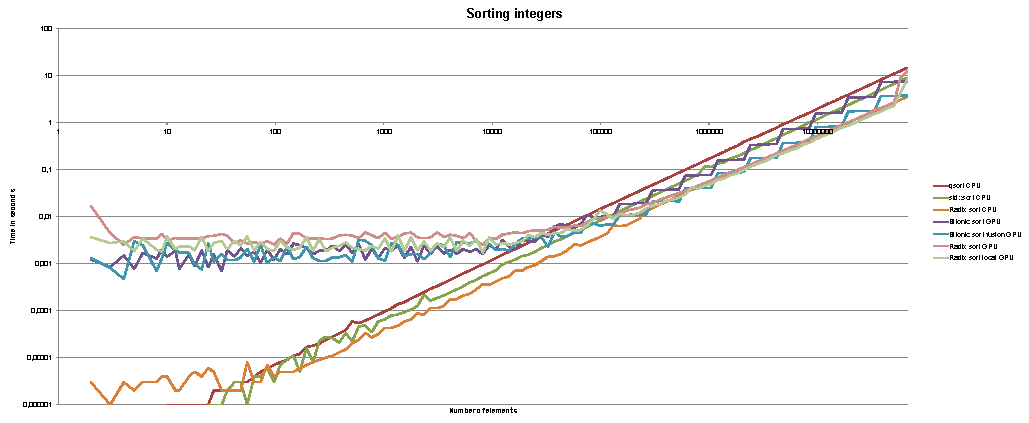
\includegraphics[width=\linewidth]{sort_chart}
\caption{Benchmark of several sort implementations. The chart is based on the benchmark data in appendix chapter \ref{sec:sort_chart_data}. Both axis are of logarithmic scale.}
\label{fig:sort_chart}
\end{figure}

\subsection{GPU Implementations}

\subsubsection{Bitonic Sort}

Many regular sorting algorithms do not fit into a GPU's massively parallel programming model by offering insufficient parallelism, requiring non-array data structures or begin based on recursion. However, a small subgroup of sorting approaches exists that fits the requirements of parallel hardware perfectly: sorting networks. A sorting network is a network of wires (one for each input) and comparators along these wires. Comparators connect two wires, compare their values and might swap them.
Finding optimal sorting networks for a given number of inputs is difficult and still subject to research. However, in 1968 K. E. Batcher presented (beside others) an approach to create sorting networks achieving good results \cite{sort_bitonic}. His idea is based on efficiently merging a bitonic sequence into a sorted sequence, hence the name bitonic sorter. A bitonic sequence is a sequence that consists of two equally long subsequences where one is sorted ascending and the other descending. As two arbitrary elements form a bitonic sequence they can be merged into a sorted sequence. As two sequences sorted in opposite order also form a bitonic sequence they can again be merged into a sorted sequence. This allows us to create sorting networks for any power of two inputs. Figure \ref{fig:bitonic_sort} shows a bitonic sorting network for 16 input elements. The created networks consist of $\mathcal{O}(n  log^2 n)$ comparators. As $\frac{n}{2}$ comparators can be executed in parallel (cf. figure \ref{fig:bitonic_sort}), the runtime complexity of a bitonic sorter would be $\mathcal{O}(log^2 n)$ on a computer with at least $\frac{n}{2}$ processing elements.

\begin{figure}
\centering
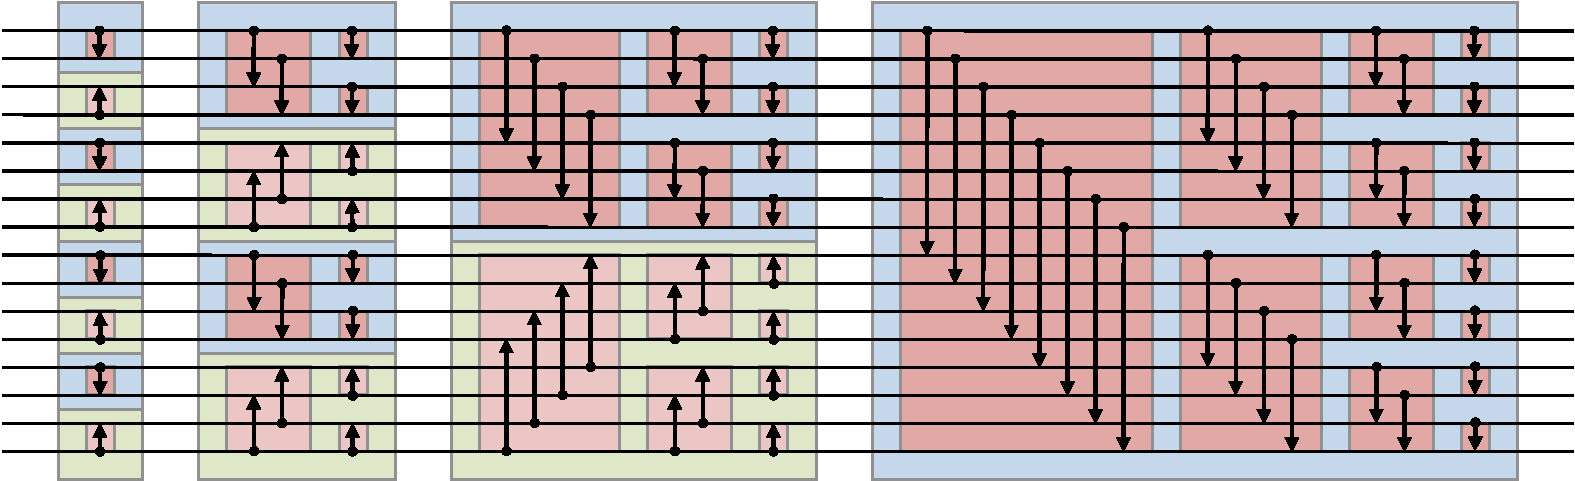
\includegraphics[width=0.8\linewidth]{bitonic_sort}
\caption{Example of a bitonic sorting network for 16 inputs \cite{wiki_bitonic_sort}. The input elements start on the left side of the network and travel through it to the right. Each arrow represents a comparator which compares the elements of the connected wires and swaps them if necessary so that the larger element is swapped to the wire the arrow points at. Each blue or green box is a separate bitonic merge receiving a bitonic sequence as input and outputting a sorted one (blue = ascending, green = descending). The red boxes contain the comparators and are equally structured. They compare the top half of the input (bitonic) sequence against the bottom half and create two bitonic sequences where each element of the upper bitonic sequence is smaller than or equal to every element in the bottom one. Further red boxes are than recursively applied to the two outputs until the sequence is sorted.}
\label{fig:bitonic_sort}
\end{figure}

Sorting inputs of any length is also possible with a bitonic sorting network. The network is constructed for the next larger power of two and all comparators affecting a wire of a (possible) input element larger than the actual input are omitted. This approach and a sample implementation is discussed in more detail in an online article by H.W. Lang \cite{sort_bitonic_arbitrary_n}. To keep the code simple the bitonic sorter implementation presented in this chapter will only focus on inputs with a power of two length.

Listing \ref{lst:sort_bitonic_host} shows the host code of a bitonic sorter implementation.

\lstset{basicstyle=\ttfamily{}\scriptsize{}}
\lstinputlisting[language=C++, caption=Host code for a bitonic sort implementation. The implementation is based on an article about experiences with OpenCL and sorting by Eric Bainville \cite{sort_bealto}., label=lst:sort_bitonic_host, firstline=106, lastline=140]{code/sort/main.cpp}
\lstset{basicstyle=\ttfamily{}}

At first the input's size is rounded up to a power of two (\lstinline!bufferSize!). A buffer read- and writable buffer is created with this size and the input data is written to it. If the input was smaller than the created buffer, the remaining part is filled with the maximum representable value of the input data type. This values should remain at the back side of the buffer during the sorting procedure and not disturb the actual input. As sorting networks are compare-and-swap-based no additional buffer is required. The input can be sorted in place.
After the buffer is set up we can begin sorting the elements. As we can see in figure \ref{fig:bitonic_sort} each column of red boxes contains half as many comparisons as inputs, which can be executed in parallel. Therefore a kernel will be enqueued for every column of red boxes. The distance between two wires of a comparator is equal across all red boxes of a column and will be called \lstinline!inc!. The red boxes itself are combined in colums of alternating blue and green boxes. The width of these boxes (the number of wires they span) will be called \lstinline!boxWidth! and determines the initial \lstinline!inc! (which is a half of the width) of their contained columns of red boxes. Furthermore the \lstinline!boxWidth! allows each comparator to derive the sorting direction (ascending or descending) from the wires' indexes.
The approach is implemented using two nested loops. The outer loop iterates the \lstinline!boxWidth!s which are powers of two starting with two until the last blue box which is equally long to the number of inputs. The inner loop iterates over the distances between two wires of the comparators inside the red box columns (\lstinline!inc!). This value starts with a half of the \lstinline!boxWidth! and decreases to the next lower power of two each loop until one.
In each iteration of the inner loop a kernel is enqueued. Arguments are the inner loops \lstinline!inc!, the other loops \lstinline!boxWidth! and the buffer with the values. The global work size is the number of comparisons of the current red box column which is a half of the input size. The local work size can be chosen freely except it must not be larger than the global one.
After all passes have been executed the sorted values can be read back from device memory.

Listing \ref{lst:sort_bitonic_kernel} shows the corresponding kernel code for the described bitonic sorter implementation.

\lstset{basicstyle=\ttfamily{}\scriptsize{}}
\lstinputlisting[language=CL, caption=OpenCL Kernel code for one iteration of a bitonic sort. The implementation is based on an article about experiences with OpenCL and sorting by Eric Bainville \cite{sort_bealto}. , label=lst:sort_bitonic_kernel,]{../src/sort/gpu/thesis/BitonicSort.cl}
\lstset{basicstyle=\ttfamily{}}

The kernel begins by calculating the index of the first wire for the comparator corresponding to the current work item. This is achieved by modifying the global id. The bits below the \lstinline!inc! bit (the lower part) stay the same. This value determines the wire index in the upper half of a red box. The bit at position \lstinline!inc! of the global id corresponds to the upper (0) or lower (1) half of the red box. This bit shall be zero to get the upper wire of the comparator. The remaining (upper) part of the global id above the \lstinline!inc! bit is a multiple of the width of a red box and therefore determines the index of the red box inside the column. The combined value is stored in \lstinline!i!.
The next step is to decide upon the sorting order of the current comparator. This can be done by looking at the bit at position \lstinline!boxWidth! of the upper wire's index. If this bit is zero, the comparator belongs to a blue box and the sorting order is ascending. Otherwise we are in a green box and have to sort descending.
Afterwards the two values at the input wires of the comparator are loaded from global memory. The positions are \lstinline!i! and \lstinline!i + inc!. If the values have to be swapped they are written back to global memory in opposite order.

Looking at the performance data in figure \ref{fig:sort_chart} we can see that the GPU bitonic sorter performs equally well as C++'s \lstinline!std::sort()!. If we look very closely we can even see that the bitonic sorter's runtime raises a bit faster than the one of the CPU sorting algorithm. This can be explained simply by their runtime complexities which are $\mathcal{O}(n log^2 n)$ for the bitonic network and $\mathcal{O}(n log n)$ for \lstinline!std::sort()!.
When profiling the code the first problem that can be noticed are the number of enqueued kernels which is 1053 for an input of $2^{26}$ elements. Furthermore, the large number of work items are quite lightweight. The latter is not a problem as such but it is important to notice that here is still space for optimization. Fortunately, both issues can be solved by combining several separate kernel invocations into a larger, heavier kernel. This is also known as kernel fusion and topic of the next chapter.


\subsubsection{Bitonic Sort using kernel fusion}

The basic concept of kernel fusion is to reduce the amount of redundant global memory loads and stores to the same locations between two or more separate kernel invocations.
Using the example of the bitonic sorting network for 16 inputs in figure \ref{fig:bitonic_sort} kernel fusion could be used to combine the kernel invocations for the second and third column of red boxes. Considering only the upper blue box, work item zero and one would load the values of wire one to three. After the first red box all four values would be stored back to global memory. On the next kernel invocation, work item zero and one would again load the same values for the following two red boxes of the same column. By combining the two separate kernel invocations into one, the redundant global memory store and load between the two kernels could be avoided.
This idea can be taken further to combine even more invocations into a single kernel. However, fusing kernels tends to making the work items heavier in resource consumption. Considering the bitonic sorting network where each work item initially had to store two values from global memory, the fused kernel (combining two invocations) would require storing four values per work item. This value increases by powers of two and therefore sets a limit to the amount of kernels that can be fused together.

Listing \ref{lst:sort_bitonic_fusion_host} shows the changes to the previous bitonic sorter host implementation.

\lstset{basicstyle=\ttfamily{}\scriptsize{}}
\lstinputlisting[language=C++, caption=Changes to the host code from listing \ref{lst:sort_bitonic_host} for a bitonic sort implementation using kernel fusion. The implementation is based on an article about experiences with OpenCL and sorting by Eric Bainville \cite{sort_bealto}., label=lst:sort_bitonic_fusion_host, firstline=157, lastline=197]{code/sort/main.cpp}
\lstset{basicstyle=\ttfamily{}}

The outer and inner loop enqueuing the kernels stay the same. However, if the increment \lstinline!inc! is large enough a fused kernel can be used which processes more than one column of red boxes with multiple increments (decreasing powers of two). The largest fused kernel being used is \lstinline!kernel16! which processes 16 input values and fuses four invocations with four different increments. Larger kernels are still possible but showed to consume to much registers to increase performance (register spilling). Nevertheless, larger kernels may be beneficial on newer hardware with more available registers. By using \lstinline!kernel16! the inner loop's \lstinline!inc! variable can be incremented to the fourth lower power of two instead of the next one, which is controlled by the \lstinline!ninc! variable. Kernels with eight, four and two inputs follow analogously. The kernel with two inputs is actually the original one used before kernel fusion.
After the appropriate kernel has been chosen it is enqueued with the same parameters as an unfused kernel. Only the number of enqueued work items decreases as each work item now processes more values.

The corresponding kernel code is based on the previous chapter in listing \ref{lst:sort_bitonic_kernel}. As several very similar kernels have to be created, the preprocessor is used to reduce redundant code.

\lstset{basicstyle=\ttfamily{}\scriptsize{}}
\lstinputlisting[language=CL, caption={OpenCL code of several kernels performing 1,2,4 or 8 iterations of a bitonic sort. The implementation is based on an article about experiences with OpenCL and sorting by Eric Bainville \cite{sort_bealto}.} , label=lst:sort_bitonic_fusion_kernel,]{../src/sort/gpu/thesis/BitonicSortFusion.cl}
\lstset{basicstyle=\ttfamily{}}

The kernel code basically starts with the \lstinline!order! procedure which orders two values (at index \lstinline!a! and \lstinline!b!) of an array \lstinline!x! either ascending or descending depending on the value of \lstinline!asc!. The \lstinline!BITONIC_SORT_FUSION! macro than declares the actual kernel plus a merge procedure. Arguments to the macro are the number of input wires the expanded kernel should process (\lstinline!lvl!) as well as the logarithm of base two for this value (\lstinline!logLvl!). Finally also the half of the \lstinline!lvl! argument has to be specified. This value cannot be calculated at it is used in token pasting and macro expansion. \\
The macro begins by declaring a merge procedure for the current number of input wires. Arguments are a pointer to the array holding the values of the input wires (\lstinline!x!) and a boolean determining the sort order (\lstinline!asc!). For the half number of input wires, comparison have to be made (cf. a larger red box in figure \ref{fig:bitonic_sort}). Then both halves of the input array are merged using two invocations of the merge procedure of the next lower level (half the current input wires). This is the actual fused part of the kernel which now processes the next two smaller red boxes sharing the same inputs as the initial red box. Although the merge procedure is recursive it cannot be implemented as such due to OpenCL not allowing recursive function calls. The reason for this is that OpenCL programs do not have a runtime stack for storing local (not \lstinline!__local!!) variables. They have to be stored in registers and therefore the maximum amount of necessary register space needed by the program has to be determinable at compile time (and will be fully allocated when the kernel is executed). The final \lstinline!merge2! procedure will not have to call any recursive merges any more. Therefore the macro \lstinline!merge1! is declared empty (recursion anchor). \\
After the merge procedure follows the actual kernel for \lstinline!lvl! number of inputs. The code is basically taken from the previous, non-fused version from the last chapter. The first adjustment made is to decrease the kernel's increment to the one of  the last fused original kernel's invocation. Furthermore, when constructing the wire index of the first value to load, not only the bit at \lstinline!inc!'s position is set to zero but \lstinline!logLvl! bits, as \lstinline!lvl! values will be loaded instead of two. These values are loaded from global memory starting at the computed start index \lstinline!i! with a stride of \lstinline!inc!. The core forms the invocation of the bitonic merge on the loaded array \footnote{As the loaded values of the input wires have to be simply sorted, it is possible to replace the bitonic merge by any kind of sorting algorithm.}. The sorted values are then written back to global memory.
Finally the macro is expanded to produce a merge procedure and a kernel for levels 2, 4, 8 and 16.

The difference in performance can be seen clearly when comparing the fused bitonic sorter against the previous implementation in figure \ref{fig:sort_chart}. For sorting $2^{26}$ elements the fused variant only requires 3.808 seconds which is roughly two times faster than the original version (7.678 seconds). This is mostly due to reduced global memory traffic by cutting down the number of enqueued kernels which has shrunken to 294 (compared with the initial 1053). In comparison to \lstinline!std::sort()! which requires 9.039 seconds this is a speedup of 2.37. \\
The implementation can still be improved by taking advantage of local memory. Eric Bainville also shows a version of the fused level four kernel using local memory in his excellent article from which most of this bitonic sort approaches are taken from \cite{sort_bealto}. The benchmarks however only show an insignificant boost (several milliseconds) in performance on the cost of a relatively complex kernel. Therefore this idea will not be covered. \\
Another idea would be to place the loaded values from the wires into local memory as local memory is accessible on a 4-byte boundary (1-byte with OpenCL extension cl\_khr\_byte\_addressable\_store). Arrays in registers can only by accessed by index at full register boundaries (16 byte) forcing the compiler to allocate more register space than the initial array requires. By placing arrays in local memory the register usage of work items could be cut down allowing higher occupancy on the cost of slower memory access. With a work group size of 256 (used in all benchmarks and the maximum of the used GPU), a level 32 kernel would already consume the full 32 KiB of local memory on the used GPU. However, when placing the array in registers, a level 32 kernel would already spill registers into global memory which is incredibly slow. Therefore a level 32 kernel might be beneficial when using local memory. Nevertheless, this approach has not been tested with the bitonic sorter. The idea is reconsidered when discussing radix sort in chapter \ref{sec:sorting_radix_local}.


\subsubsection{Radix Sort}
\label{sec:sorting_radix}

We have already discussed radix sort in the CPU implementation chapter \ref{sec:sorting_radix_cpu}. Implementing radix sort for the GPU comes down again to three steps which are executed in passes. The first step is to create a histogram for the radix of the current pass. Secondly the histogram has to be scanned and finally the input values are permuted according to the scanned histogram. 
Creating the histogram is easy. For each input element a work item is created which determines the histogram element which should be incremented. By using atomic operations which are available since OpenCL 1.1 (extension in OpenCL 1.0) the histogram can simply be stored in global memory and concurrently updated from all threads without errors. As global memory atomics are relatively slow, each work group should first compute a histogram in local memory which is then finally reduced to one in global memory.
However, this kind of histogram is of little to no use during the fully parallel permute stage. The reason for this is that every work item must be able to determine the destination address for its value independently of other threads. Although it would be possible for all work items of the same histogram bucket to obtain different destination addresses again by using atomic increments on the histogram (similar to the CPU implementation where each bucket's histogram value is incremented after writing a value to this bucket), it does not work on a GPU. Because OpenCL does not guarantee the order in which work items are executed, work items with higher global id might write values to a bucket before work items with lower id do. As a consequence the permute pass would not be stable anymore which is crucial to not ruin the permutation of a previous pass.
A solution to this problem can be found by thinking about the information a work item needs to find its correct destination address. In addition to the the start address of the region where all values of the same bucket should be written to (as in a single histogram), each work item also needs to know how many work items having a value belonging to the same bucket have a smaller global id than the current work item. This can be solved by spreading the histogram down to all individual work items. As each work item now owns a separate histogram memory consumption raises enormously. Therefore, multiple input values are processed in each work item. The histograms, after they have been created by the work items, are moved to global memory as such that the histogram entries of the same bucket across all work items lie consecutively and ascendingly in memory followed by the next group of buckets and so forth. As a result, the scan step can simply scan the whole block of histogram memory without any special cases. Therefore, the vector scan kernel developed in chapter \ref{sec:scan_vector} can be fully reused as building block for this radix sort implementation. 

Listing \ref{lst:sort_radix_host} shows the host code for an OpenCL radix sort implementation.

\lstset{basicstyle=\ttfamily{}\scriptsize{}}
\lstinputlisting[language=C++, caption=Host code for a radix sort implementation. The code is based on the radix sort sample shipped with AMD APP SDK \cite{amd_app_sdk}., label=lst:sort_radix_host, firstline=241, lastline=297]{code/sort/main.cpp}
\lstset{basicstyle=\ttfamily{}}

At the top of the source code several macros define constants. The first three should already be known from the previous CPU implementation in chapter \ref{sec:sorting_radix_cpu}. A major difference is the relatively small radix used with the GPU implementation. This is justified by the huge amount of memory required to store a histogram of $2^{RADIX}$ for each work item. New is the \lstinline!BLOCK_SIZE! constant which defines how many elements each work item processes. Its value of 32 has been determined by benchmarks and may be specific to the used GPU. The \lstinline!VECTOR_WIDTH! macro defines the width of the vector types used in the scan kernel (cf. vector scan implementation in chapter \ref{sec:scan_vector}). 
The host code stars by creating two buffers with the size of the input rounded up to be a multiple of the work group size times the \lstinline!BLOCK_SIZE!. One will be used to hold the input values at the beginning of each pass (source) and the other one will be used by the permute step to write the output values to (destination). The source buffer is initialized with the unsorted input sequence from host memory. Any free space after the written sequence is filled up with the largest representable value of the input elements' data type.
Beside the source and destination buffer a further histogram buffer is needed to store a histogram for each work item. The size of this buffer has to be rounded up to fit the input size requirements for the vector scan. 
The global work size is the number of input elements divided by \lstinline!BLOCK_SIZE! as each work item processes \lstinline!BLOCK_SIZE! values. The local work size can be chosen at will as the algorithm does not depend on local memory or work group synchronization.
After the setup is complete we can start executing several sort passes identically to the CPU variant. In each pass a histogram kernel is enqueued which calculates the per work item histograms and stores them into the histogram buffer. Arguments of the kernel are the source buffer containing the input values, the histogram buffer for writing the histograms to and the bit offset of the current pass to select the corresponding bits of the input keys. After the histograms are created and stored in global memory, the histogram buffer can be scanned. The vector scan algorithm (host and kernel) from chapter \ref{sec:scan_vector} will be used directly for this job. The scanned histograms are then input to the permute kernel which will reorder the values from the source buffer into the destination buffer. Finally the references to the source and destination buffer are swapped for the next pass.
After all passes have been executed the resulting sorted sequence can be read from the source buffer (destination buffer of the last pass).

Listing \ref{lst:sort_radix_kernel} shows the corresponding kernel code.

\lstset{basicstyle=\ttfamily{}\scriptsize{}}
\lstinputlisting[language=CL, caption=OpenCL code for the histogram and permute kernels  of a radix sort. Each work item stores it's histogram in registers. The implementation is based on the radix sort sample shipped with AMD APP SDK \cite{amd_app_sdk}. , label=lst:sort_radix_kernel, lastline=41]{../src/sort/gpu/thesis/RadixSort.cl}
\lstset{basicstyle=\ttfamily{}}

The \lstinline!Histogram! kernel begins by querying the global id of the work item and setting up a zero initialized array for holding the histogram values. Each work item then processes \lstinline!BLOCK_SIZE! elements of the input buffer. For each element the bits corresponding to the current pass' bit offset are extracted to increment the appropriate bucket of the work item's histogram. After processing the input elements has finished, the histogram is split into its buckets and moved to global memory.

The \lstinline!Permute! kernel begins with copying the scanned histogram back from global memory into registers. Each histogram bucket now contains the number of elements belonging into this bucket from work items with lower global id. Then the work item again reads in the \lstinline!BLOCK_SIZE! input elements for which the scanned histogram is now available. Each value is written to the destination buffer at the start address of the corresponding bucket for this work item. The address is incremented afterwards.

Considering performance (cf. figure \ref{fig:sort_chart}), the radix sort GPU implementation is roughly equally fast as the fused bitonic sort. When looked closely one can even see that radix sort's runtime increases a little bit slower than the one of the bitonic sorter. However, the GPU radix sort cuts off at the last few input sizes as the GPUs global memory is exhausted and the driver starts to swap GPU memory into the systems main memory. Nevertheless, the GPU implementation is far behind the CPU variant with 1.884 seconds at $2^{25}$ elements compared to 0.884 seconds on the CPU.
When profiling the kernel one can see that most of the time is spent executing and waiting for global memory requests. If we have a look at the kernel code in listing \ref{lst:sort_radix_kernel} again, we can see that the \lstinline!Histogram! kernel performs \lstinline!BLOCK_SIZE! read operations of four byte (size of uint). Furthermore adjacent work items access global memory with a stride of \lstinline!BLOCK_SIZE! times four byte. As a result each four byte value from each work item is loaded using a full memory transaction. However, on NVIDIA GPUs memory transactions always load a full memory segment of 64 or 128 words (32-bit values) \cite[p13]{nvidia_opencl_best_practices}. Global memory access should therefore be coalesced, meaning that adjacent work items should access adjacent elements in global memory. In this case, all work items can be serviced in as few memory transactions as possible. However, this is not possible in our radix sort implementation unless the \lstinline!BLOCK_SIZE! is reduced to one. Nevertheless, another way of increasing memory bandwidth utilization is to request fewer but larger pieces of memory. This approach also improves performance on AMD GPUs and will be covered in chapter \ref{sec:sorting_radix_local_vec}.
A further but more subtle issue can be seen in the disassembly of both kernels. The local (not \lstinline!__local!!) array \lstinline!uint hist[BUCKETS];! is placed in a work item's registers. However, a register's size is four words (equal to an \lstinline!uint4!). To allow indexing the array (runtime indexing into registers is not possible), the array has to be either placed strided into registers (each array element occupies only the first component of each vector register) or the compiler has to generate appropriate code to transform an index into the corresponding register address and vector component. An unorthodox but working solution is to put the array into shared memory which can be addressed at a 4-byte boundary (1-byte with OpenCL extension cl\_khr\_byte\_addressable\_store). This idea will be covered in the following chapter.

\subsubsection{Radix Sort using local memory}
\label{sec:sorting_radix_local}

Instead of placing each work item's histogram in it's own registers, local memory is used to store the array. Thus, wasted register space and instruction overhead necessary to access an array placed in registers is avoided. However, accessing local memory is usually slower and accesses might suffer from bank conflicts. This implementation will take the radix sort of the previous chapter \ref{sec:sorting_radix} and move the histogram from registers to local memory.

Listing \ref{lst:sort_radix_local_host} shows the required changes to the host code from listing \ref{lst:sort_radix_host}.

\lstset{basicstyle=\ttfamily{}\scriptsize{}}
\lstinputlisting[language=C++, caption=Changes to the host code of listing \ref{lst:sort_radix_host} for a radix sort implementation using local memory to store each thread's histogram. The implementation is based on the radix sort sample shipped with AMD APP SDK \cite{amd_app_sdk}., label=lst:sort_radix_local_host, firstline=360, lastline=366]{code/sort/main.cpp}
\lstset{basicstyle=\ttfamily{}}

As local memory is shared inside a work group, we have to allocate a block of local memory large enough to hold all histograms of all work items of a work group. The local memory needs to be allocated in both kernels.

Listing \ref{lst:sort_radix_local_kernel} shows the required changes to the kernel code from listing \ref{lst:sort_radix_kernel}.

\lstset{basicstyle=\ttfamily{}\scriptsize{}}
\lstinputlisting[language=CL, caption=Changes to the OpenCL kernel code of listing \ref{lst:sort_radix_kernel} for a radix sort implementation using local memory to store each thread's histogram. The implementation is based on the radix sort sample shipped with AMD APP SDK \cite{amd_app_sdk}., label=lst:sort_radix_local_kernel, firstline=370, lastline=389]{code/sort/main.cpp}
\lstset{basicstyle=\ttfamily{}}

Instead of declaring \lstinline!hist! as local variable inside the kernel, it is now passed as pointer to \lstinline!__local! memory as an argument to both kernels. The pointer has then to be offsetted to the current work item's histogram place. Except initialization to zero in the \lstinline!Histogram! kernel, the remaining code stays the same.

Benchmarking the changed code shows a subtle but noticeable difference in performance. The initial 1.884 seconds of the original implementation from chapter \ref{sec:sorting_radix_sort} could be reduced to 1.565 seconds, simply adjusting the code to fit better to the GPUs hardware architecture. Although this code has executed faster in the benchmarks, newer GPUs might already provide scalar registers having no troubles storing an array of scalar data types.

\subsubsection{Radix Sort using local memory and vector loads}
\label{sec:sorting_radix_local_vec}

\subsection{Existing implementations}
libCL
AMD APP SDK Samples
NVIDIA OpenCL Samples
clpp

\subsection{Conclusion}